\chapter{Optimisasi Multiobjektif}
\label{ch:multi-objective}

\begin{outcome}
\begin{itemize}
    \item Mendefinisikan masalah optimisasi multiobjektif
    \item Membahas solusi dalam konteks \emph{batas Pareto}
    \item Menjelajahi pendekatan untuk menemukan batas Pareto
    \item Menggunakan perangkat lunak untuk menyelesaikan atau menghampiri batas Pareto
\end{itemize}
\end{outcome}

\begin{quote}
\itshape Anda sedang mencari mobil bekas. Satu mobil berharga \$4{,}000 dan berusia dua belas tahun; mobil lain berharga \$9{,}000 dan berusia tiga tahun; mobil ketiga berharga \$11{,}000 dan berusia delapan tahun. Mobil ketiga dapat langsung disisihkan: mobil kedua lebih murah \emph{dan} lebih baru. Namun, di antara dua mobil pertama, tidak ada perhitungan yang dapat menetapkan pemenang: pilihannya bergantung pada seberapa bernilai satu tahun usia mobil bagi Anda, dan itu merupakan penilaian, bukan optimisasi. Optimisasi multiobjektif mempelajari tepat situasi semacam ini: menyingkirkan pilihan yang seharusnya tidak dipilih oleh siapa pun dan memetakan kompromi di antara pilihan yang tersisa.
\end{quote}

\section{Pengantar Optimisasi Multiobjektif}

Pengambil keputusan sering kali harus menyeimbangkan tujuan-tujuan yang saling bersaing. Alih-alih mengoptimalkan satu besaran, kita mencari solusi yang mengompromikan berbagai sasaran, seperti biaya dengan kualitas atau efisiensi dengan keadilan. Hal ini mengarah pada bidang \emph{optimisasi multiobjektif} (MOO), yaitu kerangka kerja untuk mengidentifikasi dan menganalisis kompromi semacam itu.

Sebagai ilustrasi, perhatikan masalah sederhana perencanaan persediaan dan produksi selama horizon tetap sebanyak \(T = 10\) periode. Misalkan \(x_t\) menyatakan jumlah yang diproduksi pada periode \(t\), \(s_t\) persediaan yang dibawa setelah periode \(t\), dan \(d_t\) permintaan yang harus dipenuhi selama periode tersebut. Sistem dimulai dengan persediaan awal sebanyak \(s_0 = 5\) unit. Biaya produksi \(c^p_t\) berubah menurut waktu, sedangkan penyimpanan persediaan menimbulkan biaya tetap per unit \(c^h\).

\textbf{Kendala keseimbangan persediaan} untuk setiap periode adalah:
\[
s_t = s_{t-1} + x_t - d_t \quad \text{untuk semua } t = 1,\ldots,T
\]

\textbf{Fungsi tujuan} (versi tujuan tunggal) adalah meminimumkan biaya total:
\[
\min \sum_{t=1}^{T} \left( c^p_t x_t + c^h s_t \right)
\]

Namun, menyimpan persediaan bukan hanya mahal; tindakan ini juga menimbulkan risiko. Produk dapat rusak, dicuri, atau menjadi usang. Untuk menangkap kekhawatiran tambahan ini, kita mendefinisikan sebuah \textbf{fungsi risiko} yang memodelkan kerugian harapan akibat persediaan yang disimpan:
\[
r(s_t) = c_r \left(1 - e^{-\beta s_t}\right)
\]
dengan \(c_r\) sebagai biaya risiko maksimum dan \(\beta\) sebagai parameter sensitivitas. Fungsi ini mula-mula tumbuh cepat, tetapi mengalami saturasi seiring bertambahnya persediaan, yang mencerminkan bahwa risiko marginal dari menyimpan lebih banyak unit berkurang berkat langkah-langkah perlindungan (misalnya asuransi dan sistem keamanan).

\begin{figure}[h]
    \centering
    % Pertahankan kurva vektor sumber, tetapi potong label rasterisasi Inggris
    % dan berikan label id-ID sebagai teks TeX yang dapat dicari.
    \begin{tikzpicture}
      \node[inner sep=0] (riskplot) {\altincludegraphics[
        width=0.72\textwidth,
        trim=18 24 0 24,
        clip
      ]{Figures/risk-plot.pdf}{Grafik fungsi risiko persediaan r(s) = c_r(1 - exp(-beta*s)) terhadap tingkat persediaan s: sebuah kurva cekung mulus yang naik tajam dari nol lalu mengalami saturasi menuju biaya risiko maksimum c_r, yang menggambarkan bahwa risiko marginal berkurang seiring bertambahnya persediaan.}};
      \node[above=1mm of riskplot,font=\normalsize] {Fungsi Risiko Persediaan};
      \node[below=1mm of riskplot,font=\small] {Tingkat Persediaan ($s$)};
      \node[left=1mm of riskplot,rotate=90,font=\small] {Biaya Risiko};
    \end{tikzpicture}
    \caption{Biaya risiko persediaan sebagai fungsi tingkat persediaan.}
\end{figure}

Kini kita menghadapi sebuah \textbf{masalah multiobjektif}: kita ingin meminimumkan biaya total sekaligus risiko maksimum yang timbul sepanjang horizon perencanaan. Kedua tujuan ini bertentangan: pengurangan risiko menuntut agar persediaan tetap rendah, yang sering kali berarti produksi harus dilakukan lebih sering dengan biaya lebih tinggi.

Untuk menjelajahi kompromi tersebut, kita menyelesaikan masalah ini berulang kali dengan berbagai batas atas persediaan (yaitu membatasi \(s_t \leq R\)), dan untuk setiap nilai kita menghitung:
\begin{itemize}
    \item Biaya total optimal (produksi + penyimpanan),
    \item Risiko maksimum yang dialami di seluruh periode, yang dihitung sebagai \( \max_t r(s_t) \).
\end{itemize}

Penyapuan ini merupakan metode kendala-$\varepsilon$, yang kita definisikan nanti dalam bab ini (Bagian~\ref{sec:pareto-frontier}). Nilai parameter dalam contoh ini bersifat ilustratif; sumber daya komputasi di akhir bab (Bagian~\ref{sec:moo-tools}), seperti \texttt{pymoo}, memudahkan Anda bereksperimen dengan instans Anda sendiri.

Grafik yang dihasilkan memperlihatkan \emph{batas Pareto} (yang didefinisikan secara tepat dalam Bagian~\ref{sec:pareto-frontier}) dari solusi-solusi tak terdominasi, yaitu solusi yang tidak memiliki solusi lain dengan biaya sekaligus risiko yang lebih rendah.

\begin{figure}[h]
    \centering
    % Pertahankan titik dan kurva vektor sumber; label id-ID ditambahkan sebagai
    % teks TeX. Sumbu sumber adalah risiko maksimum (horizontal) dan biaya
    % total (vertikal), sehingga ActualText di bawah mengikuti geometri nyata.
    \begin{tikzpicture}
      \node[inner sep=0] (paretoplot) {\altincludegraphics[
        width=0.74\textwidth,
        trim=18 24 0 24,
        clip
      ]{Figures/pareto-curve.pdf}{Kurva batas Pareto untuk masalah persediaan multiobjektif, yang menggambarkan biaya risiko maksimum pada sumbu horizontal dan biaya total pada sumbu vertikal. Kurva kompromi tak terdominasi yang menurun menunjukkan bahwa risiko yang lebih rendah hanya dapat dicapai dengan menerima biaya yang lebih tinggi.}};
      \node[above=1mm of paretoplot,font=\normalsize] {Kompromi Biaya dan Risiko Maksimum (Risiko Eksponensial)};
      \node[below=1mm of paretoplot,font=\small] {Biaya Risiko Maksimum};
      \node[left=1mm of paretoplot,rotate=90,font=\small] {Biaya Total};
    \end{tikzpicture}
    \caption{Kompromi antara biaya total dan risiko persediaan maksimum.}
\end{figure}

Contoh ini menggambarkan inti optimisasi multiobjektif: menghasilkan dan menganalisis spektrum solusi yang menawarkan berbagai keseimbangan di antara sasaran-sasaran yang saling bersaing. Dalam praktiknya, pengambil keputusan memilih di antara solusi tersebut dengan menggunakan pengetahuan bidang, batas peraturan, atau preferensi pemangku kepentingan.

\section{Optimisasi Multiobjektif dan Batas Pareto}
\label{sec:pareto-frontier}

Sekarang kita nyatakan gagasan-gagasan ini dengan tepat. Konsep utamanya adalah \emph{batas Pareto} (atau \emph{front Pareto}), yang terdiri atas semua solusi yang tidak memungkinkan satu tujuan diperbaiki tanpa memperburuk sedikitnya satu tujuan lain.

\paragraph{Contoh Pemotivasi: Produsen Furnitur}

Perhatikan sebuah produsen furnitur kelas atas yang membuat meja makan dan kursi dari kayu bocote dan sonokeling yang mahal.
Produsen tersebut menerima 960 kaki papan (bdft) bocote dan 200~bdft sonokeling per bulan. Setiap meja membutuhkan 80~bdft bocote dan 12~bdft sonokeling; setiap kursi membutuhkan 20~bdft bocote dan 10~bdft sonokeling. Misalkan \(x\) menyatakan jumlah meja dan \(y\) jumlah kursi yang diproduksi. Himpunan produksi layak \(P\) diberikan oleh:

\[
\begin{aligned}
P = \{(x,y) \in \mathbb{R}^2 :\,& 80x + 20y \le 960,\\
                                   & 12x + 10y \le 200,\\
                                   & x, y \ge 0 \}.
\end{aligned}
\]

\begin{figure}[h]
    \centering
    
    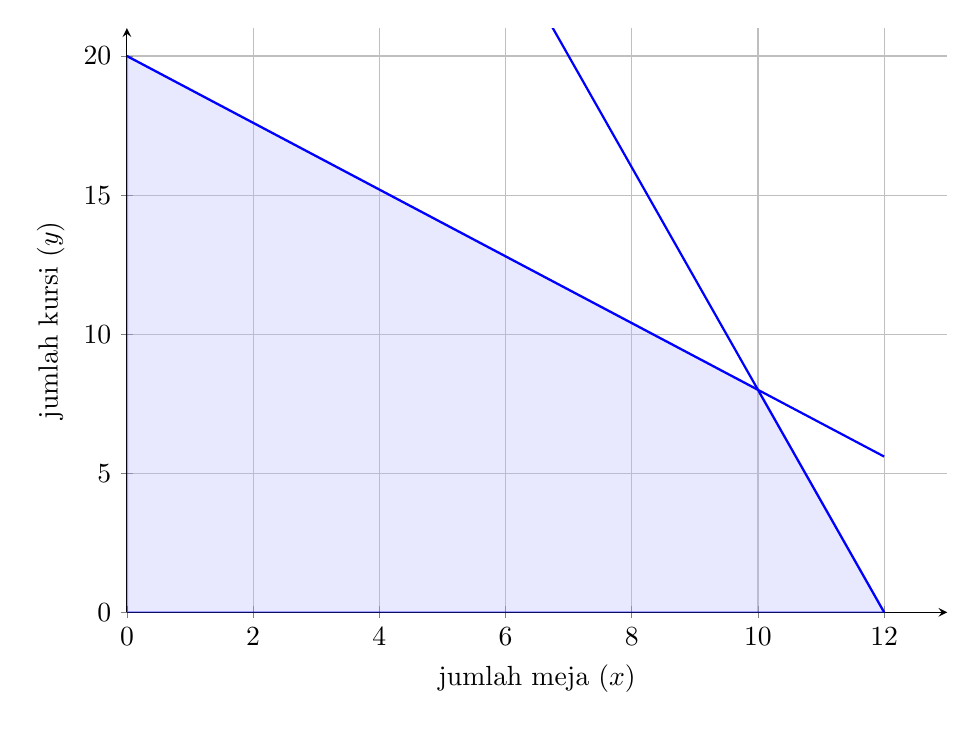
\begin{tikzpicture}
  \begin{axis}[
    xlabel={jumlah meja ($x$)},
    ylabel={jumlah kursi ($y$)},
    axis lines=left,
    xmin=0, xmax=13,
    ymin=0, ymax=21,
    xtick={0,2,4,6,8,10,12},
    ytick={0,5,10,15,20},
    width=12cm,
    height=9cm,
    grid=both,
    enlargelimits=false,
  ]

  % Wilayah layak (isian biru)
  \addplot[fill=blue!30, draw=blue, opacity = 0.3, thick] coordinates {
    (0,0)
    (0,20)
    (10,8)
    (12,0)
    (0,0)
  };

  % Garis kendala
  \addplot[domain=0:12, thick, blue] {48 - 4*x}; % 80x + 20y = 960
  \addplot[domain=0:12, thick, blue] {20 - 1.2*x}; % 12x + 10y = 200

  % Titik bilangan bulat di wilayah layak (dinonaktifkan sebagai komentar)
%  \foreach \pt in {
%    (0,0), (0,20), (10,8), (12,0),
%    (1,18), (2,16), (3,14), (4,12), (5,10), (6,8), (7,6), (8,4), (9,2), (10,0)
%  } {
%    \addplot[only marks, mark=*, mark size=2pt, black] coordinates {\pt};
%  }

  \end{axis}
\end{tikzpicture}
    \caption{Wilayah layak untuk masalah produksi furnitur.}
\end{figure}

Misalkan setiap meja menghasilkan \$8000 dan setiap kursi menghasilkan \$2000. Tujuannya adalah memaksimumkan pendapatan:

\[
\text{Maksimumkan } 8000x + 2000y \quad \text{dengan kendala } (x, y) \in P.
\]

Dengan menskalakan tujuan menjadi \(w = 4x + y\), wilayah layaknya tetap sama tetapi lebih mudah divisualisasikan. Penyelesaian LP ini menunjukkan adanya beberapa solusi optimal pada batas dari \((12, 0)\) hingga \((10, 8)\). Semua solusi tersebut menghasilkan laba yang sama, tetapi dapat berbeda menurut kriteria lain.

Sekarang, misalkan seorang manajer baru ingin meminimumkan limbah bahan, khususnya 10~bdft limbah per meja dan 2~bdft per kursi:

\[
\text{Minimumkan } 10x + 2y \quad \text{dengan kendala pendapatan maksimum}.
\]

Dengan membatasi perhatian pada batas yang optimal menurut laba dan meminimumkan limbah, kita mengidentifikasi \((10, 8)\) sebagai pilihan yang lebih disukai. Ini merupakan contoh \emph{metode leksikografis}: optimalkan tujuan primer, kemudian pertajam solusi dengan tujuan sekunder.

Sebagai alternatif, manajer mungkin bersedia mengorbankan sebagian pendapatan. Jika ia menerima sedikitnya 70\% dari laba maksimum, ia menyelesaikan:

\[
\begin{aligned}
\text{Minimumkan } &\, 10x + 2y \\
\text{dengan kendala } &\, 8000x + 2000y \ge 0.7 \times 96000,\\
&\, (x, y) \in P.
\end{aligned}
\]

\begin{figure}[h]
    \centering
            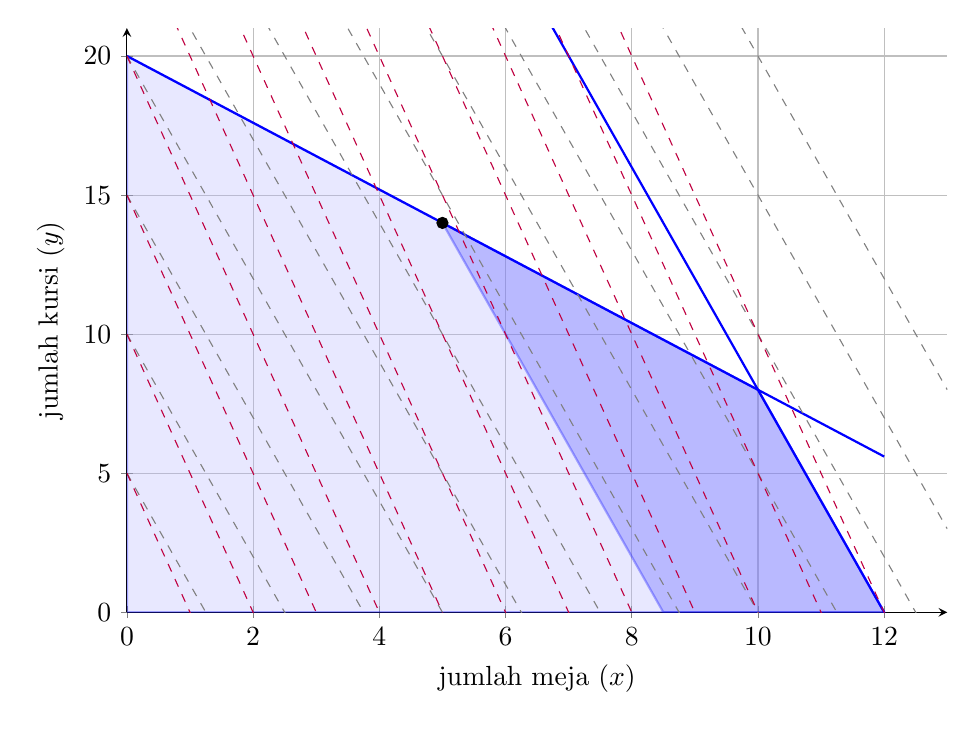
\begin{tikzpicture}
  \begin{axis}[
    xlabel={jumlah meja ($x$)},
    ylabel={jumlah kursi ($y$)},
    axis lines=left,
    xmin=0, xmax=13,
    ymin=0, ymax=21,
    xtick={0,2,4,6,8,10,12},
    ytick={0,5,10,15,20},
    width=12cm,
    height=9cm,
    grid=both,
    enlargelimits=false,
  ]

  % Wilayah layak (isian biru)
  \addplot[fill=blue!30, draw=blue, opacity = 0.3, thick] coordinates {
    (0,0)
    (0,20)
    (10,8)
    (12,0)
    (0,0)
  };
  
    \addplot[fill=blue!70, draw=blue, opacity = 0.3, thick] coordinates {
    (8.5,0)
    (5,14)
    (10,8)
    (12,0)
    (8.5,0)
  };

  % Garis kendala
  \addplot[domain=0:12, thick, blue] {48 - 4*x}; % 80x + 20y = 960
  \addplot[domain=0:12, thick, blue] {20 - 1.2*x}; % 12x + 10y = 200

  % Titik bilangan bulat di wilayah layak (dinonaktifkan sebagai komentar)
%  \foreach \pt in {
%    (0,0), (0,20), (10,8), (12,0),
%    (1,18), (2,16), (3,14), (4,12), (5,10), (6,8), (7,6), (8,4), (9,2), (10,0)
%  } {
%    \addplot[only marks, mark=*, mark size=2pt, black] coordinates {\pt};
%  }

  % Garis iso fungsi tujuan (pendapatan)
  \foreach \z in {5,10,...,60}{
    \addplot[dashed, gray, domain=0:13, samples=2] {(\z - 4*x)};
  }
  % Garis iso fungsi tujuan (limbah)
  \foreach \z in {5,10,...,60}{
    \addplot[dashed, purple, domain=0:13, samples=2] {(\z - 5*x)};
  }
  \addplot[only marks, mark=*, mark size=2pt, black] coordinates {(5,14)};
  \end{axis}
\end{tikzpicture}
    \caption{Himpunan layak dengan pendapatan yang dibatasi sedikitnya 70\% dari nilai maksimum.}
\end{figure}

Metode \emph{kendala-$\varepsilon$} ini memberikan fleksibilitas untuk menjelajahi kompromi dan menghasilkan titik-titik baru pada batas Pareto.

\paragraph{Optimalitas Pareto}

Ada banyak solusi layak, tetapi hanya sebagian yang \emph{optimal Pareto}. Sebuah solusi optimal Pareto jika tidak ada solusi layak lain yang memperbaiki satu tujuan tanpa memperburuk tujuan lain.

\begin{definition}{Optimal Pareto}
Diberikan himpunan layak \(P\) dan fungsi-fungsi tujuan \(f_i: P \to \mathbb{R}\) yang hendak \emph{dimaksimumkan}, sebuah titik \(\mathbf{x} \in P\) bersifat \emph{optimal Pareto} jika tidak ada \(\overline{\mathbf{x}} \in P\) sedemikian sehingga:
\[
\begin{aligned}
& f_i(\overline{\mathbf{x}}) > f_i(\mathbf{x}) \text{ untuk suatu } i, \\
& f_j(\overline{\mathbf{x}}) \ge f_j(\mathbf{x}) \text{ untuk semua } j \ne i.
\end{aligned}
\]
Artinya, tidak ada tujuan yang dapat diperbaiki secara tegas tanpa mengorbankan kinerja sedikitnya satu tujuan lain. \emph{Batas Pareto} adalah himpunan semua titik efisien tersebut.
\end{definition}

\begin{figure}[h]
    \centering

            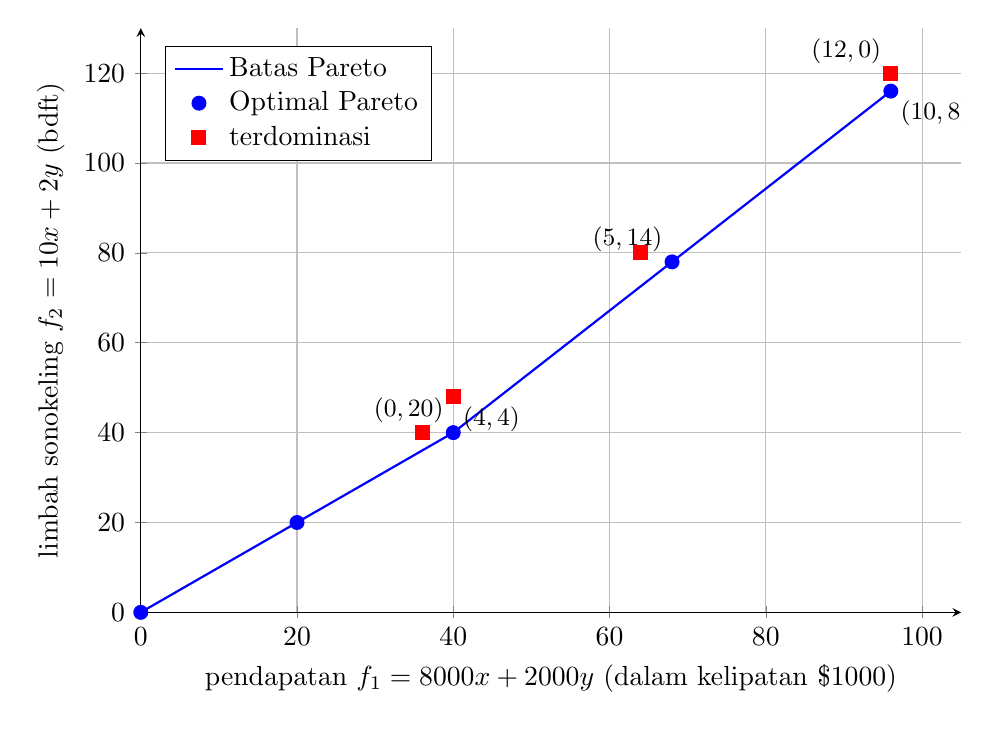
\begin{tikzpicture}
  \begin{axis}[
    xlabel={pendapatan $f_1 = 8000x + 2000y$ (dalam kelipatan \$1000)},
    ylabel={limbah sonokeling $f_2 = 10x + 2y$ (bdft)},
    axis lines=left,
    xmin=0, xmax=105,
    ymin=0, ymax=130,
    xtick={0,20,40,60,80,100},
    ytick={0,20,40,60,80,100,120},
    width=12cm,
    height=9cm,
    grid=both,
    enlargelimits=false,
    legend pos=north west,
    legend cell align=left,
  ]

  % Batas Pareto di ruang tujuan:
  % citra sisi x=0 (dari (0,0) ke (0,20)) dan sisi 12x+10y=200 (dari (0,20) ke (10,8))
  \addplot[thick, blue] coordinates {(0,0) (40,40) (96,116)};
  \addlegendentry{Batas Pareto}

  % Rencana produksi optimal Pareto: (0,0), (0,10), (0,20), (5,14), (10,8)
  \addplot[only marks, mark=*, mark size=2.5pt, blue] coordinates {
    (0,0) (20,20) (40,40) (68,78) (96,116)
  };
  \addlegendentry{Optimal Pareto}

  % Rencana produksi terdominasi: (2,10), (4,4), (8,0), (12,0)
  \addplot[only marks, mark=square*, mark size=2.5pt, red] coordinates {
    (36,40) (40,48) (64,80) (96,120)
  };
  \addlegendentry{terdominasi}

  % Beri anotasi pada rencana terpilih
  \node[above left, font=\small] at (axis cs:40,40) {$(0,20)$};
  \node[above left, font=\small] at (axis cs:68,78) {$(5,14)$};
  \node[below right, font=\small] at (axis cs:96,116) {$(10,8)$};
  \node[above left, font=\small] at (axis cs:96,120) {$(12,0)$};
  \node[below right, font=\small] at (axis cs:40,48) {$(4,4)$};

  \end{axis}
\end{tikzpicture}
    \caption{Masalah furnitur di ruang tujuan: setiap titik merupakan rencana produksi $(x,y)$ yang ditampilkan menurut pendapatannya $f_1$ (dimaksimumkan) dan limbah sonokelingnya $f_2$ (diminimumkan). Titik-titik biru tak terdominasi: tidak ada rencana layak yang menghasilkan pendapatan lebih besar tanpa menciptakan lebih banyak limbah, dan tidak ada yang menciptakan lebih sedikit limbah tanpa mengorbankan pendapatan. Titik-titik merah terdominasi; misalnya, $(12,0)$ menghasilkan pendapatan \$96{,}000 yang sama dengan $(10,8)$ tetapi membuang 120~bdft alih-alih 116, dan $(4,4)$ menyamai pendapatan $(0,20)$ dengan limbah lebih banyak. Batas tersebut terdiri atas rencana-rencana di sepanjang $x = 0$ dan di sepanjang kendala sonokeling dari $(0,20)$ hingga $(10,8)$.}
\end{figure}

\paragraph{Ringkasan Metode Optimisasi Multiobjektif}

\begin{table}[h]
\centering
\caption{Ringkasan Metode Optimisasi Multiobjektif}
\label{tab:moo-methods}
\renewcommand{\arraystretch}{1.3}
\begin{tabular}{|l|p{4.2cm}|p{3.5cm}|p{3.5cm}|}
\hline
\textbf{Metode} & \textbf{Gagasan Utama} & \textbf{Kelebihan} & \textbf{Kekurangan} \\
\hline
\textbf{Jumlah Berbobot} & Menggabungkan tujuan-tujuan menjadi satu skalar dengan jumlah berbobot & Sederhana dan efisien secara komputasi & Dapat melewatkan solusi optimal Pareto di wilayah tak konveks \\
\hline
\textbf{Leksikografis} & Memprioritaskan tujuan dalam urutan yang ketat & Sesuai dengan hierarki keputusan di dunia nyata & Tidak menjelajahi kompromi atau keseluruhan batas \\
\hline
\textbf{Kendala-Epsilon} & Mengoptimalkan satu tujuan dan memperlakukan tujuan lain sebagai kendala & Menemukan bagian tak konveks dari batas & Memerlukan penyelesaian berulang; sulit menetapkan $\varepsilon$ \\
\hline
\textbf{Pemrograman Sasaran} & Meminimumkan simpangan dari nilai sasaran & Berguna jika sasaran diketahui & Sensitif terhadap pilihan sasaran dan bobot \\
\hline
\textbf{Siku (Titik Lutut)} & Memilih titik batas tempat kompromi memburuk paling cepat & Menghasilkan satu kompromi yang seimbang & Memerlukan perhitungan batas terlebih dahulu; tidak setiap batas memiliki titik lutut yang jelas \\
\hline
\end{tabular}
\end{table}

\paragraph{Metode Skalarisasi (Jumlah Berbobot)}
Metode \emph{jumlah berbobot} mengubah masalah optimisasi multiobjektif menjadi masalah tujuan tunggal dengan menggabungkan tujuan-tujuannya secara linear.
Untuk dua tujuan $f_1(x)$ dan $f_2(x)$ (keduanya akan diminimumkan), masalah yang diskalarkan berbentuk:
\begin{align*}
\min_{x \in X} \quad & w_1 f_1(x) + w_2 f_2(x) \\
\text{d.k.} \quad & x \in X, \quad w_1, w_2 \ge 0, \quad w_1 + w_2 = 1.
\end{align*}
Di sini, $w_1$ dan $w_2$ menyatakan kepentingan relatif setiap tujuan. Memvariasikan bobot akan menelusuri bagian \emph{konveks} dari batas Pareto: setiap vektor bobot bersesuaian dengan sebuah hiperbidang pendukung pada wilayah layak di ruang tujuan.
Meskipun sederhana dan efisien secara komputasi, metode ini \emph{tidak dapat} menghasilkan titik optimal Pareto yang berada di wilayah tak konveks pada batas tersebut. Tujuan-tujuan sebaiknya dinormalisasi sebelum dibobotkan agar satuan dan skala tidak mendistorsi kompromi.

\paragraph{Metode Leksikografis}
Metode \emph{leksikografis} memeringkat tujuan dalam urutan prioritas yang ketat dan mengoptimalkannya secara berurutan: pertama-tama optimalkan tujuan terpenting, lalu optimalkan tujuan kedua pada himpunan solusi yang optimal bagi tujuan pertama, dan seterusnya. Inilah yang dilakukan produsen furnitur di atas: pertama memaksimumkan pendapatan, lalu meminimumkan limbah sonokeling di antara rencana yang optimal menurut pendapatan, sehingga terpilih $(10,8)$. Metode ini cocok untuk situasi dengan hierarki sasaran yang jelas, tetapi menghasilkan satu solusi alih-alih gambaran kompromi.

\paragraph{Pemrograman Sasaran}
\emph{Pemrograman sasaran} memasukkan nilai sasaran eksplisit untuk setiap tujuan dan mencari solusi yang meminimumkan simpangan dari sasaran-sasaran tersebut. Misalkan $g_j$ adalah sasaran yang diinginkan untuk tujuan $f_j(x)$. Perkenalkan variabel simpangan positif dan negatif $d_j^+$ dan $d_j^-$ sedemikian sehingga:
\begin{align*}
f_j(x) + d_j^- - d_j^+ = g_j, \quad d_j^+, d_j^- \ge 0.
\end{align*}
Model pemrograman sasaran \emph{berbobot} meminimumkan jumlah berbobot simpangan:
\begin{align*}
\min_{x, d^+, d^-} \quad & \sum_{j=1}^m w_j (d_j^+ + d_j^-), \\
\text{d.k.} \quad & x \in X, \; \text{dan persamaan simpangan di atas berlaku.}
\end{align*}
Bobot $w_j$ mencerminkan penalti relatif karena tidak mencapai setiap sasaran.
Dalam pemrograman sasaran \emph{preemtif} (leksikografis), tujuan diperingkat menurut prioritas dan dioptimalkan secara berurutan, sehingga sasaran berprioritas lebih tinggi dipenuhi sebaik mungkin sebelum sasaran berprioritas lebih rendah ditangani.

\paragraph{Metode Siku (Titik Lutut)}
Ketika batas Pareto digambarkan, sebagian pengambil keputusan lebih memilih satu titik kompromi tempat perbaikan lebih lanjut pada satu tujuan akan menyebabkan kerugian yang sangat tidak sebanding pada tujuan lain. \emph{Siku} atau \emph{titik lutut} ini sering ditemukan di tempat dengan kelengkungan batas terbesar.
Untuk titik-titik Pareto diskret, salah satu heuristik yang lazim adalah:
\begin{enumerate}
    \item Identifikasi solusi-solusi ekstrem (yang terbaik dalam setiap tujuan).
    \item Gambar garis lurus yang menghubungkan titik-titik ekstrem ini di ruang tujuan.
    \item Hitung jarak tegak lurus setiap titik Pareto ke garis ini.
    \item Pilih titik dengan jarak terbesar sebagai siku.
\end{enumerate}
Dalam istilah yang lebih formal, untuk batas mulus $(f_1(t), f_2(t))$, titik lutut bersesuaian dengan nilai $t$ yang memaksimumkan kelengkungan:
\begin{align*}
\kappa(t) = \frac{|f_1'(t) f_2''(t) - f_2'(t) f_1''(t)|}{\left[ (f_1'(t))^2 + (f_2'(t))^2 \right]^{3/2}}.
\end{align*}
Tidak semua front Pareto memiliki siku yang jelas, dan tujuan-tujuan sebaiknya dinormalisasi untuk menghindari bias skala.
\paragraph{Metode Kendala-Epsilon}
Metode \emph{kendala-$\varepsilon$} memilih satu tujuan sebagai sasaran optimisasi primer dan mengubah semua tujuan lain menjadi kendala dengan batas yang dapat disesuaikan.
Untuk dua tujuan $f_1(x)$ dan $f_2(x)$ (keduanya akan diminimumkan), kita dapat menyelesaikan:
\begin{align*}
\min_{x \in X} \quad & f_1(x) \\
\text{d.k.} \quad & f_2(x) \le \varepsilon, \\
& x \in X,
\end{align*}
dengan $\varepsilon$ divariasikan pada suatu rentang nilai untuk menghasilkan batas Pareto. Berbeda dari pendekatan jumlah berbobot, metode ini dapat menemukan bagian konveks maupun tak konveks dari batas tersebut. Tantangan praktis utamanya adalah memilih nilai $\varepsilon$ dan ukuran langkah yang bermakna.
Secara grafis, hal ini bersesuaian dengan penyapuan sebuah kendala horizontal (atau vertikal) melintasi wilayah tujuan layak dan pengoptimalan di dalam setiap irisan.
\subsection{Penerapan Batas Pareto}

Meskipun contoh furnitur kita berukuran kecil, optimisasi multiobjektif muncul secara alami dalam banyak bidang. Dalam setiap kasus berikut, pengambil keputusan menghadapi tujuan-tujuan yang saling bersaing dan harus memilih kompromi yang disukai di sepanjang batas Pareto.

\subsubsection{Optimisasi Portofolio}
Dalam bidang keuangan, model Markowitz klasik mencari portofolio yang mengompromikan \emph{imbal hasil harapan} dengan \emph{risiko} (varians imbal hasil). Diberikan $n$ aset dengan vektor imbal hasil harapan $\mu \in \R^n$ dan matriks kovarians $\Sigma \in \R^{n \times n}$, masalah dwi-tujuannya adalah
\[
\max \; \mu^\top w, \qquad \min \; w^\top \Sigma\, w, \qquad \text{dengan kendala} \quad \mathbf{1}^\top w = 1, \; w \geq 0.
\]
Batas Pareto masalah ini adalah \emph{batas efisien} yang terkenal: sebuah kurva pada bidang risiko--imbal hasil. Setiap portofolio pada kurva ini optimal Pareto; portofolio di bawahnya terdominasi (risiko lebih tinggi untuk imbal hasil yang sama, atau imbal hasil lebih rendah untuk risiko yang sama).

\subsubsection{Desain Rekayasa}
Insinyur mekanik dan dirgantara secara rutin menghadapi kompromi multiobjektif. Misalnya, dalam desain sayap pesawat, tujuannya dapat mencakup meminimumkan bobot (demi efisiensi bahan bakar), meminimumkan hambatan (demi kecepatan), dan meminimumkan biaya produksi, semuanya dengan tunduk pada kendala keselamatan struktural. Batas Pareto menunjukkan desain mana yang tak terdominasi, sehingga insinyur dapat memilih desain akhir yang paling sesuai dengan prioritas operasional. Kompromi serupa muncul dalam desain otomotif, tempat kenyamanan berkendara, ekonomi bahan bakar, dan kinerja akselerasi saling bersaing.

\subsubsection{Penjadwalan Staf Layanan Kesehatan}
Rumah sakit yang menjadwalkan perawat dan dokter harus menyeimbangkan biaya staf dengan mutu layanan dan keadilan beban kerja. Menambah staf pada satu giliran kerja akan mengurangi rasio pasien terhadap perawat dan kelelahan akibat lembur, tetapi meningkatkan biaya; memusatkan giliran kerja pada lebih sedikit pekerja menghemat uang, tetapi mengurangi keadilan dan meningkatkan risiko kelelahan kerja. Model dwi-tujuan yang meminimumkan biaya staf total dan, misalnya, jumlah maksimum giliran kerja yang tidak diinginkan yang ditugaskan kepada seorang perawat akan menghasilkan batas Pareto jadwal. Dengan demikian, administrator dapat melihat dengan tepat biaya setiap peningkatan keadilan, alih-alih terlebih dahulu berkomitmen pada satu pembobotan.

\subsubsection{Rantai Pasok dan Keberlanjutan}
Perusahaan semakin berupaya meminimumkan biaya sekaligus dampak lingkungan dalam rantai pasok mereka. Seorang produsen mungkin berusaha meminimumkan biaya logistik total sekaligus emisi karbon dari transportasi. Rute pengiriman yang lebih murah (misalnya dengan truk untuk jarak yang lebih jauh) dapat menghasilkan lebih banyak emisi daripada alternatif yang lebih mahal (misalnya kereta api). Batas Pareto menunjukkan kompromi yang dapat dicapai dan membantu perusahaan memenuhi sasaran keberlanjutan dengan biaya tambahan terendah.

\section{Perangkat Komputasi untuk Optimisasi Multiobjektif}
\label{sec:moo-tools}

\begin{resource}
\begin{itemize}
\item \href{https://pymoo.org/}{pymoo: Kerangka Kerja Optimisasi Multiobjektif Python}
\item \href{https://platemo.com/}{PlatEMO: Platform untuk Optimisasi Multiobjektif Evolusioner}
\end{itemize}
\end{resource}

Untuk masalah dengan lebih dari dua atau tiga tujuan, atau dengan sejumlah besar variabel keputusan, metode eksak yang dibahas di atas (jumlah berbobot, kendala-$\varepsilon$) dapat menjadi mahal secara komputasi. Dalam praktiknya, algoritma evolusioner multiobjektif (MOEA) banyak digunakan untuk menghasilkan hampiran berkualitas tinggi terhadap batas Pareto.

Beberapa algoritma terkenal tersedia untuk tujuan ini:
\begin{description}
\item[NSGA-II] (Non-dominated Sorting Genetic Algorithm II) adalah salah satu MOEA yang paling luas digunakan. Algoritma ini mempertahankan populasi solusi kandidat dan menggunakan pengurutan tak terdominasi bersama metrik jarak kerumunan untuk mempertahankan keragaman di sepanjang front Pareto. NSGA-II efektif untuk masalah dengan dua atau tiga tujuan.
\item[NSGA-III] memperluas NSGA-II untuk menangani masalah dengan banyak tujuan (empat tujuan atau lebih) dengan menggunakan arah acuan alih-alih jarak kerumunan guna mempertahankan himpunan solusi yang tersebar dengan baik di seluruh batas Pareto.
\item[MOEA/D] (Multi-Objective Evolutionary Algorithm based on Decomposition) menguraikan masalah multiobjektif menjadi kumpulan submasalah tujuan tunggal dengan menggunakan vektor bobot, lalu menyelesaikannya secara serentak. Pendekatan ini khususnya efektif ketika batas Pareto memiliki struktur yang teratur.
\end{description}

Pustaka Python \texttt{pymoo} menyediakan implementasi algoritma-algoritma ini dan banyak algoritma lainnya, beserta masalah uji bawaan, metrik kinerja, dan perangkat visualisasi untuk front Pareto. Pustaka ini menawarkan cara yang praktis untuk bereksperimen dengan optimisasi multiobjektif tanpa mengimplementasikan algoritma dari awal.

Untuk masalah kecil seperti contoh furnitur, metode kendala-$\varepsilon$ hanya memerlukan penyelesai LP biasa. Skrip PuLP berikut memaksimumkan pendapatan sambil menyapu batas limbah sonokeling, sehingga memperoleh kembali titik-titik pada batas Pareto:

\begin{lstlisting}[language=Python]
import pulp

for eps in [40, 60, 80, 100, 116]:
    prob = pulp.LpProblem("furnitur", pulp.LpMaximize)
    x = pulp.LpVariable("meja", lowBound=0)
    y = pulp.LpVariable("kursi", lowBound=0)
    prob += 8000*x + 2000*y            # pendapatan (tujuan utama)
    prob += 80*x + 20*y <= 960         # bocote
    prob += 12*x + 10*y <= 200         # sonokeling
    prob += 10*x + 2*y <= eps          # limbah <= epsilon
    prob.solve(pulp.PULP_CBC_CMD(msg=0))
    print(f"eps={eps}: x={x.value():.2f}, y={y.value():.2f}, "
          f"pendapatan={pulp.value(prob.objective):.0f}")
\end{lstlisting}

Penyapuan $\varepsilon$ dari 40 hingga 116 menelusuri batas dari rencana $(0,20)$ dengan pendapatan \$40{,}000 hingga $(10,8)$ dengan pendapatan \$96{,}000, melewati rencana pecahan seperti $x \approx 5.26$, $y \approx 13.68$ dengan pendapatan \$69{,}474 pada $\varepsilon = 80$.

\section{Latihan}

\exgroup{Pemanasan}

\begin{ex}{Mendefinisikan Optimalitas Pareto}{}
\stars{1}\label{ex:pareto-def}
Definisikan \emph{optimalitas Pareto} untuk masalah minimisasi multiobjektif dengan dua tujuan.
\exrefs{Bagian~\ref{sec:pareto-frontier}}
\end{ex}

\begin{ex}{Menemukan Desain Terdominasi}{}
\stars{1}\label{ex:moo-dominance}
Lima kontrak pemasok dinilai menurut dua tujuan yang keduanya akan diminimumkan: $f_1$ (biaya, dalam kelipatan \$1000) dan $f_2$ (waktu pengiriman, dalam hari).

\begin{center}
\begin{tabular}{c|ccccc}
Kontrak & G & H & I & J & K \\\hline
$f_1$    & 2 & 4 & 5 & 7 & 6 \\
$f_2$    & 9 & 7 & 8 & 3 & 5 \\
\end{tabular}
\par\captionof{table}{Biaya dan waktu pengiriman untuk kelima kontrak pemasok.}\label{tab:multi-objective-optimization_updated-tab01}% tab-num-auto

\end{center}

\begin{enumerate}
\item Kontrak mana yang terdominasi, dan oleh kontrak mana?
\item Cantumkan batas Pareto menurut urutan $f_1$ yang meningkat.
\item Benar atau salah: kontrak yang merupakan peminimum unik $f_1$ tidak akan pernah terdominasi. Jelaskan.
\end{enumerate}
\exrefs{Bagian~\ref{sec:pareto-frontier}, Latihan~\ref{ex:pareto-table}}
\end{ex}

\begin{ex}{Menghitung Skor Jumlah Berbobot}{}
\stars{1}\label{ex:moo-weighted-scores}
Dengan menggunakan tabel kontrak dari Latihan~\ref{ex:moo-dominance}, bentuk skor berbobot $S = w_1 f_1 + w_2 f_2$ (kedua tujuan diminimumkan, sehingga skor terendah menang).
\begin{enumerate}
\item Untuk $(w_1, w_2) = (0.6, 0.4)$, hitung kelima skor dan identifikasi kontrak pemenang.
\item Ulangi untuk $(w_1, w_2) = (0.2, 0.8)$. Mengapa pemenangnya berubah?
\item Kontrak I terdominasi oleh kontrak H. Tunjukkan bahwa untuk setiap pilihan bobot $w_1, w_2 > 0$, skor kontrak I secara tegas lebih buruk daripada H, sehingga titik terdominasi tidak pernah dapat memenangi jumlah berbobot dengan bobot positif.
\end{enumerate}
\exrefs{Bagian~\ref{sec:pareto-frontier}}
\end{ex}

\exgroup{Soal inti}

\begin{ex}{Batas Pareto, Jumlah Berbobot, dan Kendala-$\varepsilon$}{}
\stars{2}\label{ex:pareto-table}
Perhatikan himpunan layak desain berikut dengan dua tujuan yang akan diminimumkan: $f_1$ (biaya) dan $f_2$ (emisi).
Tabel ini mencantumkan enam \emph{kandidat} dari suatu studi desain; sebagian mungkin terdominasi di dalam himpunan ini.

\begin{center}
\begin{tabular}{c|cccccc}
Desain & A & B & C & D & E & F \\\hline
$f_1$  & 6 & 4 & 7 & 3 & 5 & 10 \\
$f_2$  & 5 & 8 & 4 & 6 & 6 & 3 \\
\end{tabular}
\par\captionof{table}{Biaya dan emisi untuk keenam desain kandidat.}\label{tab:multi-objective-optimization_updated-tab02}% tab-num-auto

\end{center}

\begin{enumerate}
\item Identifikasi semua desain \textbf{optimal Pareto} dari $\{A,\ldots,F\}$ dan cantumkan batas Paretonya.
\vspace{2cm}

\item Misalkan kita menggunakan \emph{jumlah berbobot} dengan bobot $(\alpha,1-\alpha)$, $\alpha\in[0,1]$. Desain mana yang dapat diperoleh sebagai solusi optimal untuk suatu $\alpha$? Berikan alasan singkat.

\vspace{2cm}

\item Dengan menggunakan metode kendala-$\varepsilon$ yang meminimumkan $f_1$ dengan syarat $f_2\le \varepsilon$, berikan nilai $\varepsilon$ yang mencapai desain pada batas yang \emph{tidak dapat diperoleh} oleh jumlah berbobot mana pun (jika ada), atau jelaskan mengapa semua titik batas dapat dicapai dengan jumlah berbobot.

\vspace{2cm}

\item Buat sketsa (dengan tangan) titik-titik pada bidang $(f_1,f_2)$, tandai titik-titik terdominasi, dan gambar batas Pareto dengan anak panah yang menunjukkan arah perbaikan.

\vspace{6cm}
\end{enumerate}
\exrefs{Bagian~\ref{sec:pareto-frontier}, Tabel~\ref{tab:moo-methods}}
\end{ex}

\begin{ex}{Metode Jumlah Berbobot}{}
\stars{2}\label{ex:weighted-sum-projects}
Seorang perencana kota sedang mengevaluasi tiga proyek peningkatan jalan. Setiap proyek memiliki biaya (yang akan diminimumkan) dan skor aksesibilitas (yang akan dimaksimumkan):

\begin{center}
\begin{tabular}{c|c|c}
\textbf{Proyek} & \textbf{Biaya (juta \$)} & \textbf{Skor Aksesibilitas} \\
\hline
P1 & 2 & 7 \\
P2 & 5 & 9 \\
P3 & 3 & 6 \\
\end{tabular}
\par\captionof{table}{Biaya dan skor aksesibilitas untuk setiap proyek peningkatan jalan.}\label{tab:multi-objective-optimization_updated-tab03}% tab-num-auto

\end{center}

Kita merumuskan ulang sebagai masalah minimisasi dengan tujuan $f_1 = \text{biaya}$ dan $f_2 = -\text{aksesibilitas}$ (sehingga keduanya diminimumkan).

\begin{enumerate}
\item Proyek mana yang optimal Pareto? Berikan alasan untuk jawaban Anda.
\item Dengan metode jumlah berbobot menggunakan bobot $w_1 = 0.5$ untuk biaya dan $w_2 = 0.5$ untuk aksesibilitas negatif, proyek mana yang dipilih?
\item Apakah ada himpunan bobot yang akan memilih proyek P3? Jelaskan.
\end{enumerate}
\exrefs{Bagian~\ref{sec:pareto-frontier}}
\end{ex}

\begin{ex}{Metode Kendala-Epsilon}{}
\stars{2}\label{ex:eps-constraint-lp}
Perhatikan sebuah program linear dwi-tujuan:
\[
\min \; (f_1(\mathbf{x}), \; f_2(\mathbf{x})) = (x_1 + 2x_2, \; 3x_1 + x_2)
\]
dengan kendala $x_1 + x_2 \geq 4$, $x_1 \leq 5$, $x_2 \leq 5$, dan $x_1, x_2 \geq 0$.

\begin{enumerate}
\item Terapkan metode kendala-$\varepsilon$: minimumkan $f_1$ dengan syarat $f_2 \leq \varepsilon$. Tuliskan LP tujuan tunggal yang dihasilkan.
\item Temukan solusi optimal untuk $\varepsilon = 10$ dan untuk $\varepsilon = 6$. Apakah kedua solusi optimal Pareto?
\item Jelaskan apa yang terjadi ketika $\varepsilon$ berkurang dari suatu nilai besar menuju $f_2^*$ (nilai minimum $f_2$ saja).
\end{enumerate}
\exrefs{Bagian~\ref{sec:pareto-frontier}, Bagian~\ref{sec:moo-tools}}
\end{ex}

\begin{ex}{Kendala-Epsilon secara Manual}{}
\stars{2}\label{ex:eps-triangle}
Perhatikan dua tujuan yang akan \emph{dimaksimumkan}, $f_1 = 3x_1 + x_2$ dan $f_2 = x_1 + 3x_2$, di atas segitiga
\[
X = \{(x_1, x_2) \geq 0 : x_1 + x_2 \leq 6\}.
\]
\begin{enumerate}
\item Evaluasi kedua tujuan pada ketiga titik sudut $X$. Titik sudut mana yang memaksimumkan $f_1$ saja? Mana yang memaksimumkan $f_2$ saja?
\item Terapkan metode kendala-$\varepsilon$: maksimumkan $f_1$ dengan syarat $f_2 \geq \varepsilon$ dan $x \in X$, untuk setiap $\varepsilon \in \{6, 10, 14, 18\}$. Selesaikan setiap LP secara manual (secara grafis, atau dengan memeriksa titik-titik sudut wilayah yang diiris) dan tabulasikan $(x_1, x_2, f_1, f_2)$.
\item Bagian mana dari batas $X$ yang merupakan batas Pareto di ruang keputusan? Berapa laju kompromi antara $f_1$ dan $f_2$ di sepanjang batas tersebut?
\item Apa yang terjadi jika $\varepsilon > 18$?
\end{enumerate}
\exrefs{Bagian~\ref{sec:pareto-frontier}, Bagian~\ref{sec:moo-tools}}
\end{ex}

\begin{ex}{Analisis Kompromi}{}
\stars{2}\label{ex:tradeoff-analysis}
Sebuah perusahaan manufaktur menghadapi dua tujuan yang bertentangan: meminimumkan biaya produksi ($f_1$) dan meminimumkan emisi lingkungan ($f_2$). Setelah menyelesaikan serangkaian masalah jumlah berbobot, ditemukan solusi-solusi optimal Pareto berikut:

\begin{center}
\begin{tabular}{c|c|c}
\textbf{Solusi} & $f_1$ \textbf{(Biaya, kelipatan \$1000)} & $f_2$ \textbf{(Emisi, ton)} \\
\hline
S1 & 40 & 20 \\
S2 & 45 & 14 \\
S3 & 55 & 10 \\
S4 & 70 & 8 \\
\end{tabular}
\par\captionof{table}{Solusi optimal Pareto yang ditemukan dengan metode jumlah berbobot.}\label{tab:multi-objective-optimization_updated-tab04}% tab-num-auto

\end{center}

\begin{enumerate}
\item Gambarkan titik-titik ini di ruang tujuan. Gambar batas Paretonya.
\item Hitung tingkat substitusi marginal (rasio kompromi) di antara setiap pasangan solusi yang berurutan. Lompatan biaya mana yang memberikan pengurangan emisi terbesar per dolar?
\item Jika perusahaan bersedia membelanjakan paling banyak \$50{,}000, solusi optimal Pareto mana yang harus dipilih?
\end{enumerate}
\exrefs{Bagian~\ref{sec:pareto-frontier}}
\end{ex}

\exgroup{Konsep dan kaitan}

\begin{ex}{Hal yang Tidak Dapat Dilihat oleh Jumlah Berbobot}{}
\stars{2}\label{ex:nonconvex-weights}
Sebuah studi desain menghasilkan tepat tiga hasil optimal Pareto di ruang tujuan, dengan kedua tujuan diminimumkan:
\[
P = (0, 4), \qquad Q = (3, 3), \qquad R = (4, 0).
\]
\begin{enumerate}
\item Verifikasi bahwa tidak satu pun dari titik-titik ini mendominasi yang lain.
\item Untuk bobot $(\alpha, 1-\alpha)$ dengan $\alpha \in [0,1]$, tuliskan skor berbobot setiap titik sebagai fungsi $\alpha$ dan tunjukkan bahwa $\min\{4\alpha,\, 4 - 4\alpha\} \leq 2 < 3$ untuk setiap $\alpha$. Simpulkan bahwa $Q$ tidak pernah menjadi optimum jumlah berbobot, bahkan sebagai nilai seri.
\item Jelaskan hasilnya secara geometris: titik mana yang berada pada selubung konveks bawah dari $\{P, Q, R\}$, dan mengapa setiap jumlah berbobot bersesuaian dengan garis pendukung selubung tersebut? Kaitkan jawaban Anda dengan entri ``Kekurangan'' untuk metode jumlah berbobot pada Tabel~\ref{tab:moo-methods}.
\item Sebutkan metode dari Tabel~\ref{tab:moo-methods} yang dapat memperoleh kembali $Q$, dan berikan nilai parameter tertentu yang berhasil.
\end{enumerate}
\exrefs{Bagian~\ref{sec:pareto-frontier}, Tabel~\ref{tab:moo-methods}}
\end{ex}

\begin{ex}{Leksikografis versus Jumlah Berbobot}{}
\stars{2}\label{ex:lex-vs-weighted}
Dalam contoh furnitur di Bagian~\ref{sec:pareto-frontier}, metode leksikografis (pertama memaksimumkan pendapatan, lalu meminimumkan limbah di antara rencana yang optimal menurut pendapatan) memilih $(10, 8)$.
\begin{enumerate}
\item Jumlah berbobot yang menempatkan seluruh bobot pada pendapatan ($\alpha = 1$) hanya memaksimumkan $8000x + 2000y$. Rencana mana yang optimal dalam kasus ini, dan mengapa hal ini tidak mereproduksi jawaban leksikografis?
\item Nyatakan bahwa sembarang bobot $\alpha < 1$ yang cukup dekat dengan $1$ akan memilih tepat $(10, 8)$: bobot kecil pada limbah berfungsi sebagai pemutus seri di antara rencana yang optimal menurut pendapatan, tetapi terlalu kecil untuk membenarkan pengorbanan pendapatan. (Latihan~\ref{ex:furniture-weights} menghitung ambang batas tepatnya.)
\item Kapan kedua metode ini secara umum memberikan hasil yang sama? Jelaskan mengapa untuk program linear dengan titik sudut yang berjumlah hingga selalu ada bobot yang cukup ekstrem untuk mereproduksi solusi leksikografis, dan uraikan secara informal apa yang dapat keliru jika bobot pada tujuan sekunder tidak cukup kecil.
\end{enumerate}
\exrefs{Bagian~\ref{sec:pareto-frontier}, Tabel~\ref{tab:moo-methods}}
\end{ex}

\exgroup{Soal tantangan}

\begin{ex}{Bobot yang Memilih Setiap Titik Sudut}{}
\stars{3}\label{ex:furniture-weights}
Kembali ke contoh furnitur pada Bagian~\ref{sec:pareto-frontier}. Ukur pendapatan dalam ribuan dolar, sehingga tujuannya adalah $f_1 = 8x + 2y$ (dimaksimumkan) dan $f_2 = 10x + 2y$ (diminimumkan, limbah dalam bdft). Metode jumlah berbobot menyelesaikan
\[
\max_{(x,y) \in P} \; \alpha f_1(x,y) - (1-\alpha) f_2(x,y), \qquad \alpha \in [0,1].
\]
\begin{enumerate}
\item Optimum selalu dicapai pada sebuah titik sudut $P$: $(0,0)$, $(0,20)$, $(10,8)$, atau $(12,0)$. Tuliskan nilai tujuan berbobot pada setiap titik sudut sebagai fungsi linear $\alpha$.
\item Untuk setiap titik sudut optimal Pareto, temukan interval tepat $\alpha$ tempat titik tersebut optimal, dan berikan nilai titik pisah $\alpha$.
\item Apa yang optimal tepat pada setiap titik pisah, dan pada $\alpha = 1$? Jelaskan mengapa titik sudut terdominasi $(12,0)$ muncul pada $\alpha = 1$ dan apa maknanya bagi penggunaan bobot nol.
\item Ulangi bagian (2) dengan pendapatan dalam dolar tanpa penskalaan ($f_1 = 8000x + 2000y$). Di mana letak titik-titik pisahnya sekarang? Apa yang ditunjukkan hal ini mengenai normalisasi tujuan sebelum memilih bobot?
\end{enumerate}
\exrefs{Bagian~\ref{sec:pareto-frontier}, Tabel~\ref{tab:moo-methods}}
\end{ex}

\subsubsection*{Solusi Terpilih}

\begin{solution}(Latihan~\ref{ex:pareto-def})
Untuk masalah yang meminimumkan $f_1$ dan $f_2$ pada himpunan layak $P$, sebuah titik $\mathbf{x} \in P$ bersifat \emph{optimal Pareto} jika tidak ada $\overline{\mathbf{x}} \in P$ dengan $f_i(\overline{\mathbf{x}}) \leq f_i(\mathbf{x})$ untuk kedua $i = 1, 2$ dan $f_i(\overline{\mathbf{x}}) < f_i(\mathbf{x})$ untuk sedikitnya satu $i$. Dengan kata lain: tidak ada titik layak lain yang sedikitnya sama baik dalam kedua tujuan dan secara tegas lebih baik dalam salah satunya.
\end{solution}

\begin{solution}(Latihan~\ref{ex:pareto-table})
(1) Bandingkan pasangan-pasangan untuk menentukan dominasi (kedua tujuan diminimumkan). $D = (3,6)$ mendominasi $B = (4,8)$. $E = (5,6)$ terdominasi oleh $D$ ($3 \leq 5$, $6 \leq 6$). $A = (6,5)$ tidak terdominasi. $C = (7,4)$ tidak terdominasi. $F = (10,3)$ tidak terdominasi. Batas Paretonya adalah $\{D, A, C, F\}$ dengan vektor tujuan $(3,6), (6,5), (7,4), (10,3)$.

(2) Sebuah desain menjadi optimum jumlah berbobot untuk suatu $\alpha$ tepat ketika desain tersebut berada pada selubung konveks kiri bawah dari titik-titik batas. Dengan menggambarkan $(3,6), (6,5), (7,4), (10,3)$, selubung konveks bawah dibentuk oleh $D$, $C$, dan $F$, sedangkan $A$ berada di atasnya: $D$ ($f_1$ terbaik) dan $F$ ($f_2$ terbaik) selalu dapat diperoleh, dan $C$ berada pada selubung di antara keduanya, tetapi $A$ terletak di atas ruas dari $D$ ke $C$ (periksa kemiringan: dari $D$ ke $C$, $\Delta = (4, -2)$; $A$ pada $(6,5)$ dibandingkan dengan nilai ruas $6 - \tfrac{2}{4}(6-3) = 4.5 < 5$), sehingga $A$ tidak dapat diperoleh dengan jumlah berbobot apa pun.

(3) Pilih $\varepsilon = 5$: meminimumkan $f_1$ dengan syarat $f_2 \leq 5$ akan memilih $A = (6,5)$, yaitu titik batas yang tidak dapat dicapai dengan jumlah berbobot.
\end{solution}

\begin{solution}(Latihan~\ref{ex:eps-triangle})
(1) Pada $(0,0)$: $(f_1, f_2) = (0,0)$. Pada $(6,0)$: $(18, 6)$. Pada $(0,6)$: $(6, 18)$. Jadi, $(6,0)$ memaksimumkan $f_1$ saja dan $(0,6)$ memaksimumkan $f_2$ saja.

(2) Untuk $\varepsilon > 6$, kendala $x_1 + 3x_2 \geq \varepsilon$ aktif pada optimum, dan solusinya berada di perpotongan kendala tersebut dengan sisi $x_1 + x_2 = 6$: penyelesaian kedua persamaan menghasilkan $x_2 = (\varepsilon - 6)/2$, $x_1 = (18 - \varepsilon)/2$.
\begin{center}
\begin{tabular}{c|cccc}
$\varepsilon$ & $x_1$ & $x_2$ & $f_1$ & $f_2$ \\\hline
6  & 6 & 0 & 18 & 6 \\
10 & 4 & 2 & 14 & 10 \\
14 & 2 & 4 & 10 & 14 \\
18 & 0 & 6 & 6  & 18 \\
\end{tabular}
\par\captionof{table}{Solusi masalah kendala-$\varepsilon$ ketika $\varepsilon$ bervariasi.}\label{tab:multi-objective-optimization_updated-tab05}% tab-num-auto

\end{center}

(3) Setiap solusi memiliki tepat $f_2 = \varepsilon$ dan $f_1$ terbesar yang dimungkinkan dengan batas itu, sehingga setiap solusi optimal Pareto. Batasnya adalah sisi $x_1 + x_2 = 6$ dari $(6,0)$ hingga $(0,6)$: parameterisasi dengan $x_2 = t$ menghasilkan $f_1 = 18 - 2t$ dan $f_2 = 6 + 2t$, yaitu kompromi satu banding satu di antara kedua tujuan.

(4) Nilai maksimum $f_2$ di atas $X$ adalah $18$, sehingga untuk $\varepsilon > 18$ LP berkendala tersebut tidak layak; penyapuan harus berhenti di sana.
\end{solution}

\begin{solution}(Latihan~\ref{ex:furniture-weights})
(1) Tujuan berbobot $\alpha(8x + 2y) - (1-\alpha)(10x + 2y)$ pada setiap titik sudut:
\[
(0,0): 0, \qquad
(0,20): 80\alpha - 40, \qquad
(10,8): 212\alpha - 116, \qquad
(12,0): 216\alpha - 120.
\]

(2) Nilai optimal merupakan selubung atas dari keempat fungsi linear $\alpha$ ini. Dengan membandingkan pasangan: $(0,20)$ mengalahkan $(0,0)$ jika dan hanya jika $80\alpha - 40 \geq 0$, yaitu $\alpha \geq \tfrac12$; $(10,8)$ mengalahkan $(0,20)$ jika dan hanya jika $212\alpha - 116 \geq 80\alpha - 40$, yaitu $132\alpha \geq 76$, yakni $\alpha \geq \tfrac{19}{33} \approx 0.576$; dan $(10,8)$ mengalahkan $(12,0)$ jika dan hanya jika $4 \geq 4\alpha$, yang berlaku untuk semua $\alpha \leq 1$. Jadi,
\[
(0,0) \text{ optimal untuk } \alpha \in [0, \tfrac12], \qquad
(0,20) \text{ untuk } \alpha \in [\tfrac12, \tfrac{19}{33}], \qquad
(10,8) \text{ untuk } \alpha \in [\tfrac{19}{33}, 1].
\]
Penyapuan numerik mengonfirmasi peralihannya: $\alpha = 0.5757$ menghasilkan $(0,20)$ dan $\alpha = 0.5758$ menghasilkan $(10,8)$.

(3) Pada $\alpha = \tfrac12$, seluruh sisi $x = 0$ optimal (setiap rencana $(0,y)$ berskor $0$ di sana); pada $\alpha = \tfrac{19}{33}$, seluruh sisi sonokeling dari $(0,20)$ hingga $(10,8)$ optimal. Pada $\alpha = 1$, limbah diabaikan, sehingga semua rencana yang optimal menurut pendapatan, yaitu sisi dari $(10,8)$ hingga $(12,0)$, bersifat optimal, termasuk rencana terdominasi $(12,0)$. Jumlah berbobot dengan bobot nol dapat menghasilkan titik yang tidak optimal Pareto; sembarang bobot positif pada limbah memutus seri untuk memenangkan $(10,8)$.

(4) Dengan $f_1 = 8000x + 2000y$, perbandingan yang sama menghasilkan titik pisah $\alpha = \tfrac{1}{1001} \approx 0.001$ dan $\alpha = \tfrac{19}{14019} \approx 0.00136$: hampir setiap bobot memilih $(10,8)$. Ketika tujuan berada pada skala yang sangat berbeda, bobot kehilangan makna yang dimaksudkan, sehingga tujuan harus dinormalisasi sebelum dibobotkan (Bagian~\ref{sec:pareto-frontier}).
\end{solution}
